\subsection{Exact points: the dose law of loam}
The worked example of Part~8 of the guide on its curve: the share of each irrigation millimetre that drains, against the dose applied at each event.
\begin{center}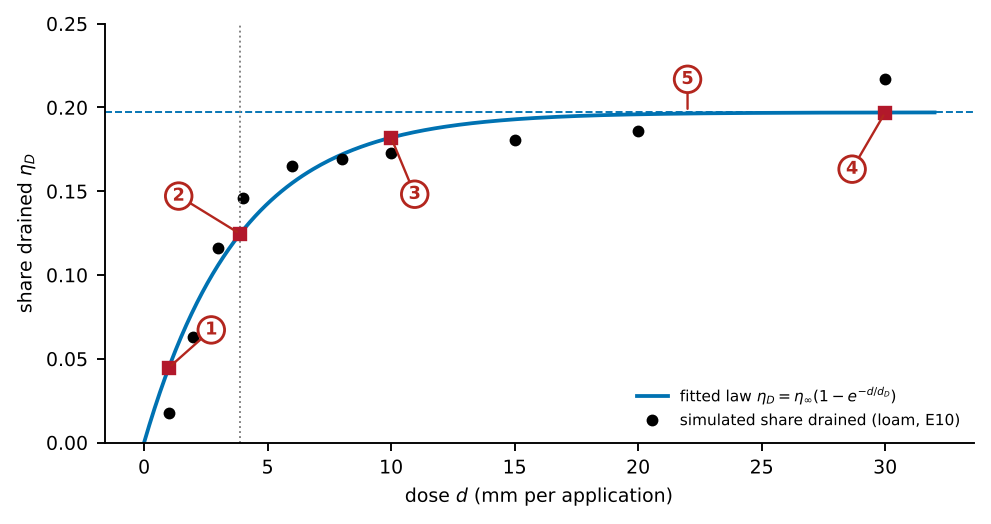
\includegraphics[width=0.92\textwidth]{../figures/paper4/ex_dose.png}\end{center}
\textbf{What the numbered labels point to, with the exact values.}
\begin{enumerate}[nosep,label=\protect\circled{\arabic*}]
\item $d=1$\,mm: $1-e^{-1/3.9}=0.23$; $\eta_D=0.045$. A small dose is used the same day and almost nothing drains.
\item $d=d_D=3.9$\,mm: by definition $\eta_D=\eta_\infty(1-e^{-1})=0.63\,\eta_\infty=0.125$.
\item $d=10$\,mm: $\eta_D=0.182$, already 92\,\% of the plateau.
\item $d=30$\,mm: $\eta_D=0.197$, practically the plateau.
\item The plateau $\eta_\infty=0.197$ of loam: the share of a large dose that drains, set by the race between drainage and uptake.
\end{enumerate}
\textbf{How the exact points are obtained from the data.} The black dots come from experiment E10 (\texttt{E10\_Amount\_Timing\_Soil}): the irrigated runs of loam are grouped by the dose per event (column \texttt{set\_dose\_mm\_per\_event}, 1 to 30\,mm, all irrigation windows pooled), and for each dose the summed extra drainage over the rainfed twin (E0) is divided by the summed irrigation. They are stored in \nolinkurl{p4_fig5_dose.csv}. The curve is the least-squares fit of the two parameters $\eta_\infty$ and $d_D$ (\texttt{scipy.optimize.curve\_fit} in \nolinkurl{p4_reach.py}); the fitted values and their standard errors are in \nolinkurl{p4_numbers.json} under \texttt{constants.dose\_fit}. The workbook sheet \texttt{EQ\_P4\_dose} evaluates the law at any dose.
